\documentclass[brazil, bsc, 10pt]{beamer}
%\usetheme{default}
\usecolortheme{dove}
\usepackage[utf8]{inputenc}
\usepackage{lastpage}		
\usepackage{indentfirst}
\usepackage[alf]{abntex2cite}	
\usepackage{tikz}
\usepackage{circuitikz}
\usepackage{graphicx}
\usetikzlibrary{arrows.meta, positioning, shapes, fit}
\usepackage{lipsum}
\usepackage[english]{babel}
\usepackage[linesnumbered]{algorithm2e}
\setbeamertemplate{navigation symbols}{}
\usepackage{listings}
\usepackage{minted}

\tikzstyle{box} = [rectangle, rounded corners, minimum width=3cm, minimum height=1cm, text centered, draw=black, fill=gray!20]
\tikzstyle{arrow} = [thick, ->, >=stealth]

\title[Intro]{I/O Patterns and Bottlenecks in Deep Learning Workloads}
\author[Hugen]{
  Pablo Alessandro Hugen\inst{1}
}

\institute[UFRGS]{
  \inst{1}%
  Institute of Informatics -- UFRGS\\
}

\date[2024]{
  Comp. Sys. Perf. Analysis 2025/2
}

\logo{%
  \makebox[0.95\paperwidth]{%
      
\includegraphics[width=2cm,keepaspectratio]{images/logo-ufrgs.png}
    \hfill%
    
\includegraphics[width=2cm,keepaspectratio]{images/logo-ppgc.png}
  }%
}
\AtBeginSection[] {
  \begin{frame}<beamer>{Content}
    \tableofcontents[currentsection]
  \end{frame}
}

\begin{document}

\frame{\titlepage}
\logo{}

\section{Introduction}

\subsection{Context}

\begin{frame}
	\frametitle{Context}

	\begin{block}{}
		\begin{itemize}
			\item Recent growing interest in optimizations for Machine Learning/Deep Learning
			      training and inference methods.
			\item Used in various fields: LLMs, Image reconition and classifications, and so on.
			\item Large models often need very large HPC infraestructures for
			      processing the insane amount of training data.
			\item The performance of the storage and I/O subsystem of HPC systems is critical

		\end{itemize}
	\end{block}
\end{frame}

\begin{frame}
	\frametitle{Context}

	\begin{block}{}
		\begin{itemize}
			\item Traditional HPC workloads are characterized by large, sequential data access \cite{characterizing_ml_io_workloads}.
			      \begin{itemize}
				      \item Simulations which saves the state at the end or in checkpoints
			      \end{itemize}

			\item In contrast, ML workloads generate small, random reads across numerous files \cite{characterizing_ml_io_workloads}.

			\item Large amounts of data (far greater than system memory) + random read pattern = lot of page faults and cache misses (VERY BAD)
		\end{itemize}
	\end{block}
\end{frame}

\begin{frame}
	\frametitle{Context}
	\begin{center}
		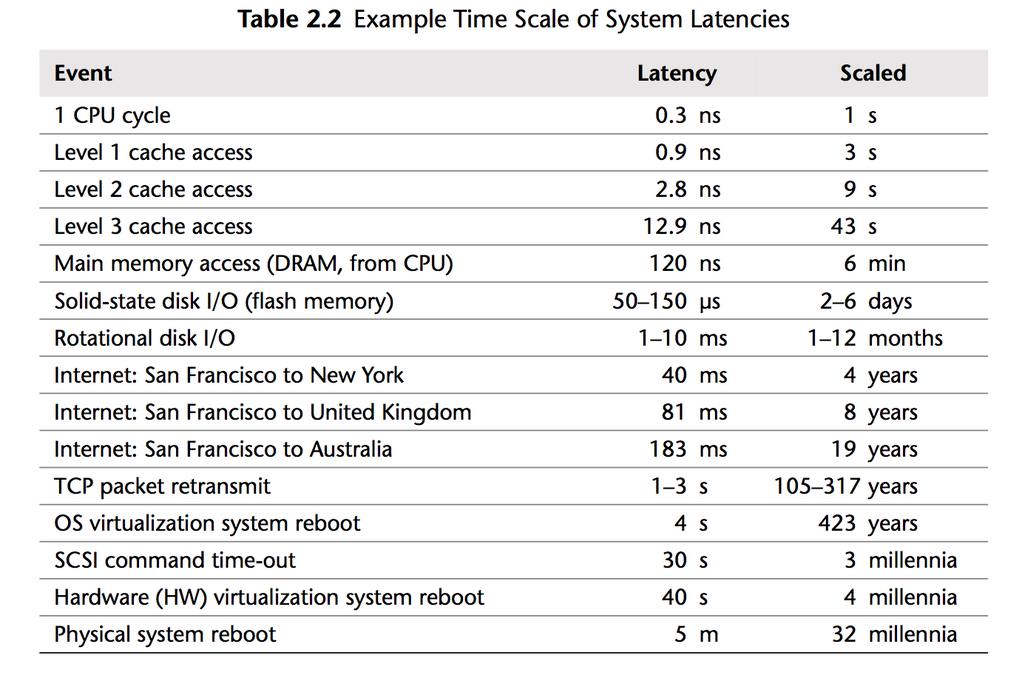
\includegraphics[width=0.8\textwidth]{./images/latencies.png}
	\end{center}
\end{frame}

\begin{frame}
	\frametitle{Context}

	\begin{block}{}
		\begin{itemize}
			\item At Large Scale Distributed DL Workloads, IO can take roughly 85\% of the \emph{training} time \cite{clairvoyant_prefetching_for_distributed_ml_io}.
			\item And training is often one of the most expensive parts of the pipeline \cite{io_machine_learning_applications}.
		\end{itemize}
	\end{block}
	\begin{center}
		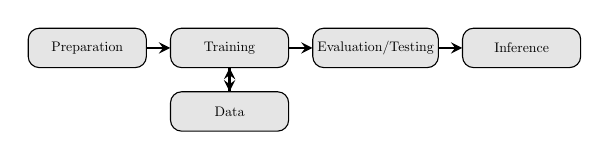
\begin{tikzpicture}[
				node distance=0.6cm,
				auto,
				scale=0.5,
				transform shape
			]

			\node[box] (prep) {Preparation};
			\node[box, right=of prep] (train) {Training};
			\node[box, right=of train] (eval) {Evaluation/Testing};
			\node[box, right=of eval] (infer) {Inference};

			% New "Data" node below Training
			\node[box, below=of train] (data) {Data};

			\draw[arrow] (prep) -- (train);
			\draw[arrow] (train) -- (eval);
			\draw[arrow] (eval) -- (infer);

			% Arrows between Training and Data
			% One arrow from Training to Data
			\draw[arrow] (train.south) -- (data.north);
			% One arrow from Data to Training
			\draw[arrow] (data.north) -- (train.south);

			% Alternatively, a single bidirectional arrow:
			% \draw[bidirectional_arrow] (train) -- (data); 
		\end{tikzpicture}
	\end{center}
\end{frame}


\subsection{Objectives}

\begin{frame}
	\frametitle{Objectives}
	\begin{block}{General:}
		Understand \alert{patterns in I/O operations and possible bottlenecks} in common
		Machine Learning workloads
	\end{block}
	\begin{block}{Especifics:}
		\begin{itemize}
			\item \textbf{Disk throughput}: Understand how disk throughput varies in training between epochs, checkpoints and when the number of training processes varies.

			\item \textbf{GPU usage}: Know how the GPU usage (\%) behaves in those scenarios.
		\end{itemize}
	\end{block}
\end{frame}

\subsection{Justification}

\begin{frame}
	\frametitle{Justification}
	\begin{block}{}
		\begin{itemize}
			\item By understanding those patterns and possible bottlenecks I hope to \alert{find some ideas and directions for further work}.
		\end{itemize}
	\end{block}
\end{frame}

\subsection{Related Works}

\begin{frame}
	\frametitle{Related Work}
	\begin{block}{\citeonline{io_machine_learning_applications}}
		Surveys literature from 2019 to 2024 on the I/O challenges, patterns, and optimizations for machine learning applications on high-performance computing systems to identify gaps for future research.
	\end{block}

	\begin{block}{\citeonline{analyzing_the_io_patterns}}
		This paper presents a methodology for analyzing the input/output (I/O) patterns of deep learning applications on high-performance computing (HPC) systems, applying it to codes using TensorFlow2 and PyTorch with the MNIST and CIFAR-10 datasets to understand performance bottlenecks.
	\end{block}
\end{frame}

\begin{frame}
	\frametitle{Related Work}
	\begin{block}{\citeonline{understanding_and_leveraging_the_io_patterns_of_emerging_ml_analytics}}
		This paper discusses the complex I/O patterns and challenges of emerging machine learning workflows used for large-scale scientific data analysis, proposes methods to optimize data transfers, and demonstrates performance gains with a medical application case study.
	\end{block}

	\begin{block}{\citeonline{characterizing_ml_io_workloads}}
		This paper presents an in-depth I/O characterization of over 23,000 machine learning jobs from a one-year period on the Summit supercomputer, using the Darshan tracing tool to analyze how their behavior varies across different scientific domains and workload scales.
	\end{block}
\end{frame}

\section{Methodology (so far)}

\begin{frame}
	\frametitle{Methodology (so far)}
	\begin{block}{}
		\begin{itemize}
			\item Simulation: dlio\_benchmark \cite{dlio_benchmark}.
			\item The experiments are available at \url{https://github.com/HpcResearchLaboratory/perf_2025}.
			      \begin{itemize}
				      \item Custom workloads
				      \item dlio\_benchmark (python venv :(, will try to use nix shell )
				      \item Slurm script to perform all benchmarks
			      \end{itemize}
		\end{itemize}
	\end{block}
\end{frame}

\begin{frame}
	\frametitle{Methodology (so far)}
	\begin{block}{System}
		\begin{table}[h!]
			\centering
			\caption{System Specifications}
			\label{tab:system_specs}
			\resizebox{\textwidth}{!}{%
				\begin{tabular}{|l|l|}
					\hline
					\textbf{Component} & \textbf{Specification}               \\ \hline
					CPU                & 4x ARM Neoverse-V2 (288 cores total) \\ \hline
					Memory (RAM)       & 857 GiB                              \\ \hline
					GPU                & 4x NVIDIA GH200 (120GB each)         \\ \hline
					Storage            & 1.8 TB NVME                          \\ \hline
				\end{tabular}%
			}
		\end{table}
	\end{block}
\end{frame}

\begin{frame}
	\frametitle{Methodology (so far)}
	\begin{block}{Workloads}
		\begin{table}[h!]
			\centering
			\caption{Workflow Configuration Summary}
			\label{tab:workflow_summary}
			\resizebox{\textwidth}{!}{%
				\begin{tabular}{|l|l|l|l|}
					\hline
					\textbf{Model Name}     & \textbf{Framework Name} & \textbf{Epochs} & \textbf{Checkpoints Enabled}      \\ \hline
					cosmoflow\_h100\_custom & tensorflow              & 1               & No                                \\ \hline
					default\_custom         & pytorch                 & 10              & No                                \\ \hline
					dlrm\_custom            & pytorch                 & 3               & Yes (every 2 steps)               \\ \hline
					unet3d\_h100\_custom    & pytorch                 & 5               & Yes (after epoch 5, then every 2) \\ \hline
				\end{tabular}%
			}
		\end{table}
	\end{block}
\end{frame}

\begin{frame}
	\frametitle{Methodology (so far)}
	\begin{block}{Experimental project}
		\begin{itemize}
			\item \textbf{Input variables:} \# of epochs, \# of processes
			\item \textbf{Response variables:} Accelerator Usage (AU), I/O Throughput
		\end{itemize}
	\end{block}
\end{frame}

\begin{frame}
	\frametitle{Methodology (so far)}
	\begin{table}[h!]
		\centering
		\caption{Experimental setup}
		\label{tab:exp_setup}
		\renewcommand{\arraystretch}{0.7} % Command to reduce row height
		\resizebox{0.5\textwidth}{!}{%
			\begin{tabular}{|l|c|c|c|}
				\hline
				\textbf{Model} & \textbf{Epochs} & \textbf{Procs.} & \textbf{Run} \\ \hline
				cosmoflow      & 1               & 1               & N            \\ \hline
				cosmoflow      & 1               & 2               & N            \\ \hline
				cosmoflow      & 1               & 4               & N            \\ \hline
				cosmoflow      & 1               & 6               & N            \\ \hline
				cosmoflow      & 1               & 8               & N            \\ \hline
				default        & 10              & 1               & Y            \\ \hline
				default        & 10              & 2               & Y            \\ \hline
				default        & 10              & 4               & Y            \\ \hline
				default        & 10              & 6               & Y            \\ \hline
				default        & 10              & 8               & Y            \\ \hline
				dlrm           & 3               & 1               & Y            \\ \hline
				dlrm           & 3               & 2               & Y            \\ \hline
				dlrm           & 3               & 4               & Y            \\ \hline
				dlrm           & 3               & 6               & N            \\ \hline
				dlrm           & 3               & 8               & N            \\ \hline
				unet3d         & 5               & 1               & Y            \\ \hline
				unet3d         & 5               & 2               & Y            \\ \hline
				unet3d         & 5               & 4               & Y            \\ \hline
				unet3d         & 5               & 6               & Y            \\ \hline
				unet3d         & 5               & 8               & Y            \\ \hline
			\end{tabular}%
		}
	\end{table}
\end{frame}

\section{Results (so far)}

\begin{frame}
	\frametitle{Accelerator Usage vs. Number of Processes}
	\begin{figure}
		\centering
		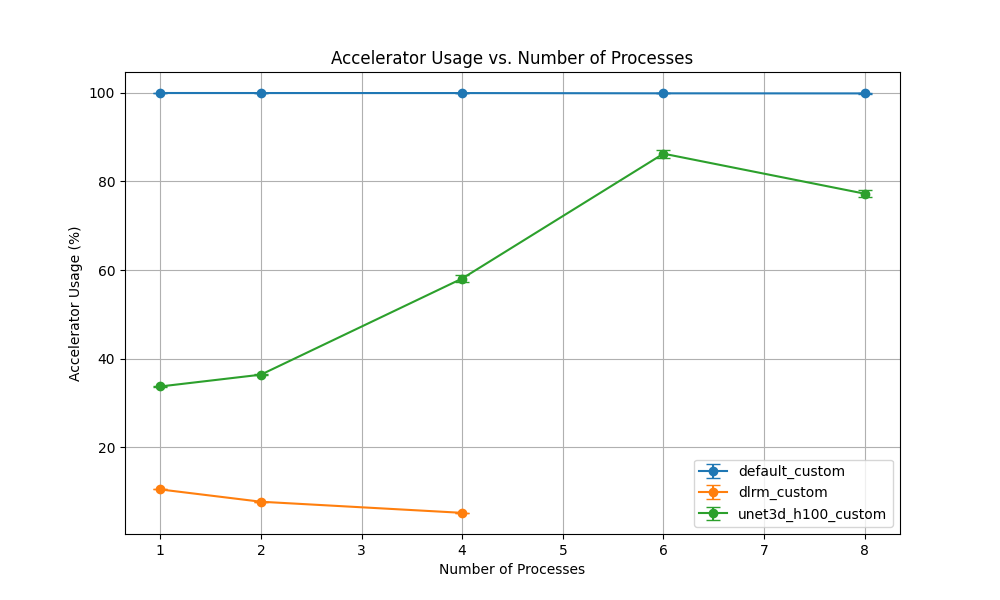
\includegraphics[width=0.9\textwidth]{images/au.png}
		\caption{Accelerator usage for different models and number of processes.}
	\end{figure}
\end{frame}

\begin{frame}
	\frametitle{I/O Throughput vs. Number of Processes}
	\begin{figure}
		\centering
		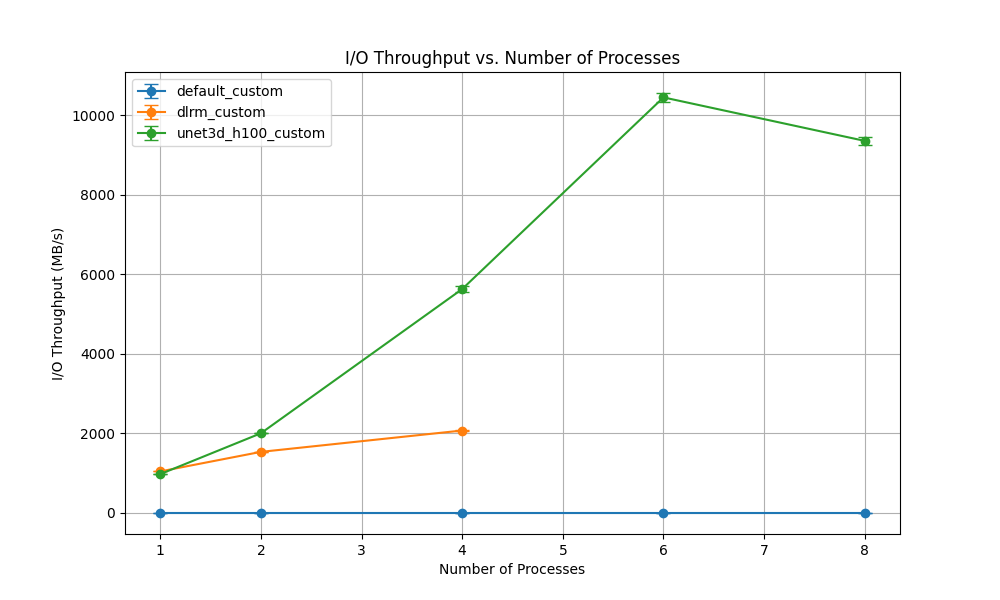
\includegraphics[width=0.9\textwidth]{images/io.png}
		\caption{I/O throughput for different models and number of processes.}
	\end{figure}
\end{frame}


\begin{frame}[allowframebreaks]
	\frametitle{Bibliography}
	\bibliography{references}
\end{frame}

\end{document}
